\section{Étude dynamique du pendule à N maillons}

\subsection{Modélisation du pendule simple (un maillon)}

Nous commençons par l’étude du pendule simple, constitué d’un seul maillon de longueur \( l \), de masse \( m \), soumis à la gravité. Son mouvement est entièrement décrit par un angle \( \theta(t) \), mesuré entre la verticale et la tige. L'équation différentielle régissant son mouvement est :

\[
\frac{d^2\theta}{dt^2} + \frac{g}{l} \sin(\theta) = 0,
\]

où \( g \) est l’accélération due à la gravité. Pour de petites oscillations, on peut linéariser cette équation en approximant \( \sin(\theta) \approx \theta \), ce qui donne une fréquence propre \( f = \frac{1}{2\pi} \sqrt{\frac{g}{l}} \).

Nous avons implémenté une fonction qui, pour un angle initial \( \theta_0 \), calcule la période moyenne du pendule à l’aide de différents schémas d’intégration numérique. La fréquence associée est ensuite calculée en faisant l’inverse de cette période. La figure \ref{fig:simple_pendulum} illustre l’évolution de cette fréquence en fonction de \( \theta_0 \), mettant en évidence le fait que la fréquence devient quasi constante pour des petites amplitudes, en accord avec la théorie linéarisée.

\begin{figure}[H]
    \centering
    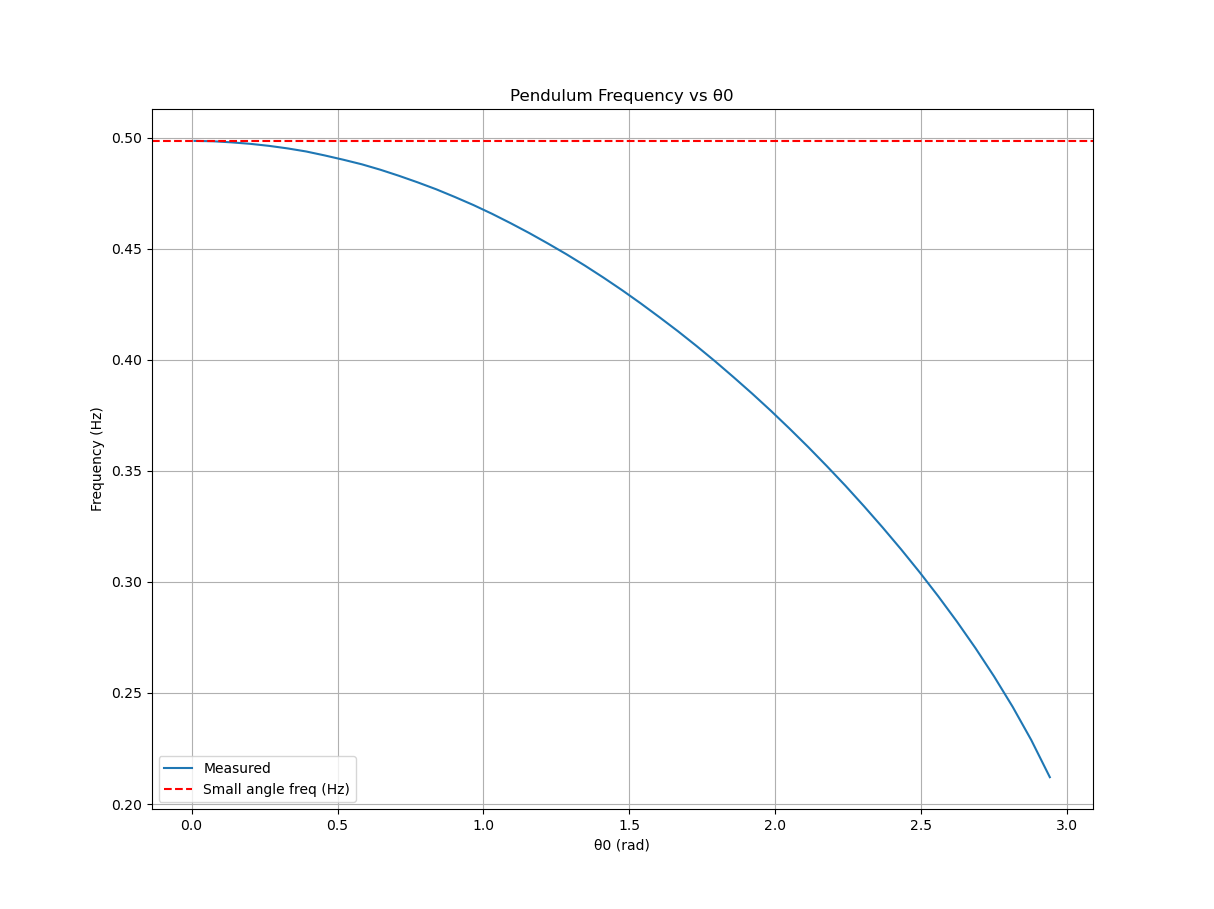
\includegraphics[width=0.5\linewidth]{img/Simple_pendulum_frequency.png}
    \caption{Fréquence d’oscillation du pendule simple en fonction de l’angle initial \( \theta_0 \). La fréquence tend vers \( \sqrt{g/l}/(2\pi) \) pour les petites oscillations.}
    \label{fig:simple_pendulum}
\end{figure}

\subsection{Modélisation du pendule double (deux maillons)}

Nous étudions ensuite le pendule double, système dynamique constitué de deux tiges de longueurs \( l_1 \) et \( l_2 \), de masses respectives \( m_1 \) et \( m_2 \), articulées en série. Ce système est modélisé par deux angles \( \theta_1(t) \) et \( \theta_2(t) \), correspondant aux positions des deux maillons. Les équations du mouvement sont obtenues par application des lois de la mécanique.

Ce système présente un comportement chaotique : de petites variations dans les conditions initiales peuvent conduire à des trajectoires radicalement différentes. Cette sensibilité est illustrée par la figure \ref{fig:double_pendulum}, où l’on observe la trajectoire de l’extrémité du second maillon pour des conditions initiales légèrement différentes.

\begin{figure}[H]
    \centering
    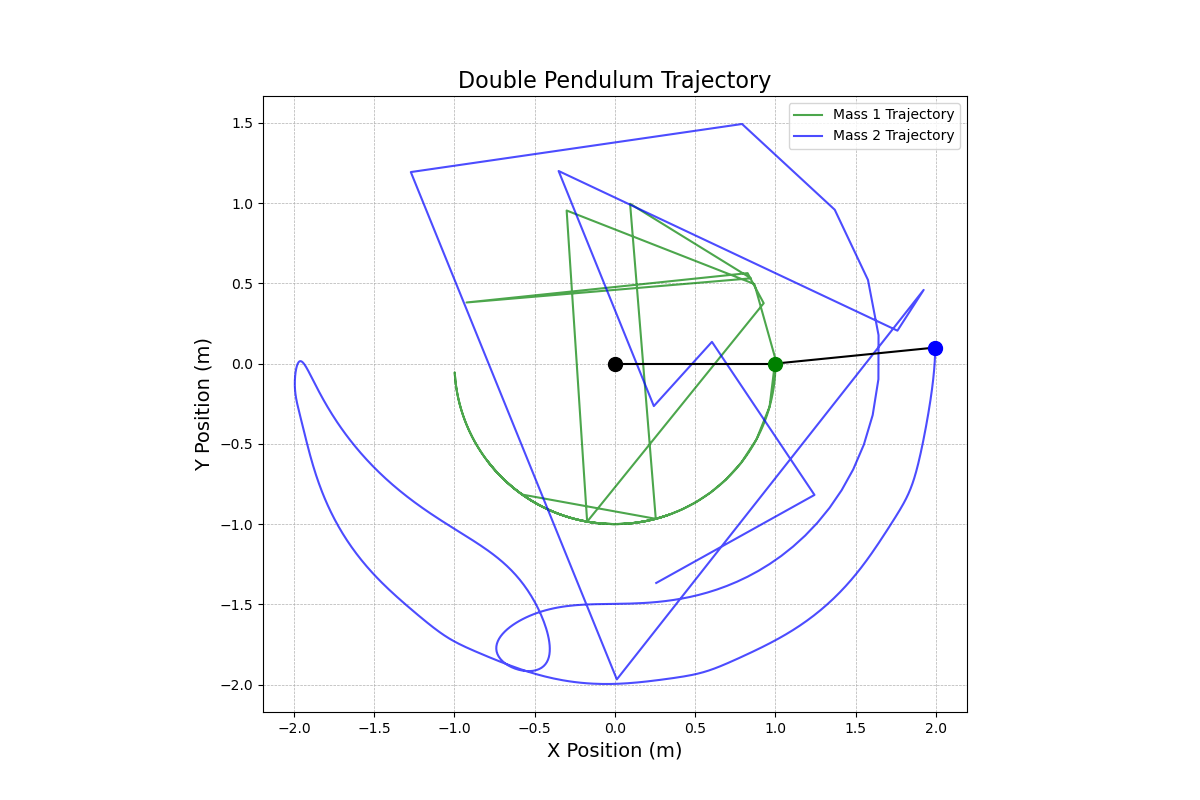
\includegraphics[width=0.6\linewidth]{img/Double_pendulum_motion.png}
    \caption{Trajectoires de l’extrémité du pendule double pour des conditions initiales proches. Les divergences soulignent le comportement chaotique du système.}
    \label{fig:double_pendulum}
\end{figure}

\subsection{Temps de premier retournement}

Pour quantifier le comportement chaotique, une méthode consiste à mesurer le \textit{temps de premier retournement}, c’est-à-dire le temps mis par le pendule pour effectuer un demi-tour complet à partir de sa position initiale. Nous avons conçu une fonction qui détecte ce moment en resolvant les equations du mouvement. En effectuant cette mesure pour un grand nombre de conditions initiales, nous avons pu générer une carte de couleurs représentant le temps de retournement, illustrée en figure \ref{fig:first_flip}.

\begin{figure}[H]
    \centering
    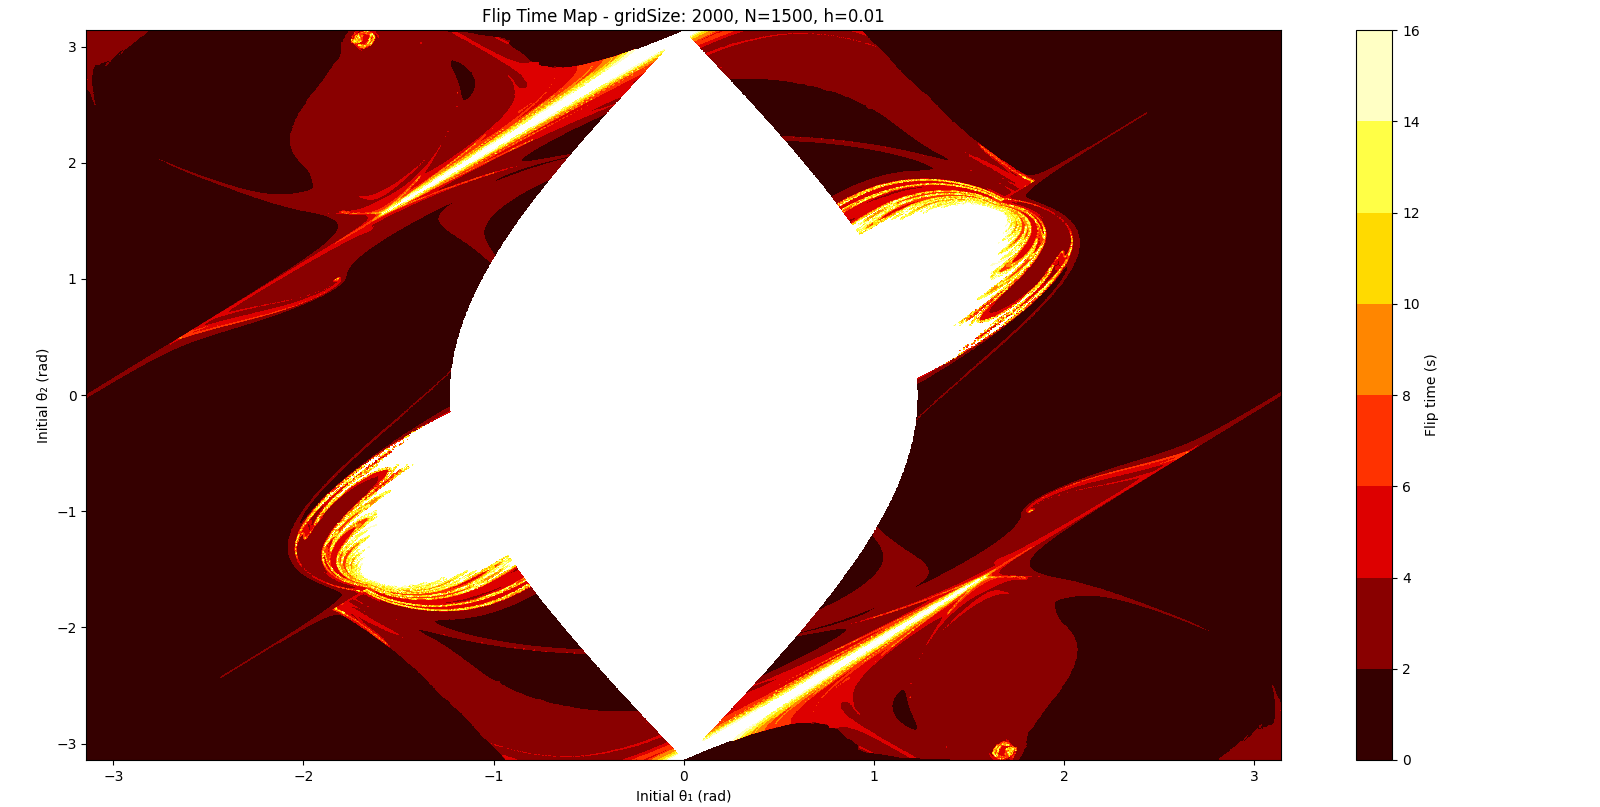
\includegraphics[width=0.75\linewidth]{img/First_flip_map.png}
    \caption{Carte du temps de premier retournement en fonction des conditions initiales \( \theta_1 \) et \( \theta_2 \). Les variations brutales de couleurs trahissent la complexité du système.}
    \label{fig:first_flip}
\end{figure}
